\documentclass{beamer}


\usepackage{amssymb,amsmath}
\usepackage{graphicx}
\usepackage{url}
\usepackage{color}
\usepackage{relsize}		% For \smaller
\usepackage{url}			% For \url
\usepackage{epstopdf}	% Included EPS files automatically converted to PDF to include with pdflatex
\usepackage{pagenote}[continuous,page]

%For MindMaps
% \usepackage{tikz}%
% \usetikzlibrary{mindmap,trees,arrows}%

%%% Color Definitions %%%%%%%%%%%%%%%%%%%%%%%%%%%%%%%%%%%%%%%%%%%%%%%%%%%%%%%%%
%\definecolor{bordercol}{RGB}{40,40,40}
%\definecolor{headercol1}{RGB}{186,215,230}
%\definecolor{headercol2}{RGB}{80,80,80}
%\definecolor{headerfontcol}{RGB}{0,0,0}
%\definecolor{boxcolor}{RGB}{186,215,230}

%%% Save space in lists. Use this after the opening of the list %%%%%%%%%%%%%%%%
%\newcommand{\compresslist}{
%	\setlength{\itemsep}{1pt}
%	\setlength{\parskip}{0pt}
%	\setlength{\parsep}{0pt}
%}

%\setbeameroption{show notes on top}

% You should run 'pdflatex' TWICE, because of TOC issues.

% Rename this file.  A common temptation for first-time slide makers
% is to name it something like ``my_talk.tex'' or
% ``john_doe_talk.tex'' or even ``discrete_math_seminar_talk.tex''.
% You really won't like any of these titles the second time you give a
% talk.  Try naming your tex file something more descriptive, like
% ``riemann_hypothesis_short_proof_talk.tex''.  Even better (in case
% you recycle 99% of a talk, but still want to change a little, and
% retain copies of each), how about
% ``riemann_hypothesis_short_proof_MIT-Colloquium.2000-01-01.tex''?

\mode<presentation>
{
  % A tip: pick a theme you like first, and THEN modify the color theme, and then add math content.
  % Warsaw is the theme selected by default in Beamer's installation sample files.

  %%%%%%%%%%%%%%%%%%%%%%%%%%%% THEME
  %\usetheme{Madrid}		% No subsection
  \usetheme{AnnArbor}  % Subsection on top, no color


  %\usetheme{Antibes}
  %\usetheme{Bergen}
  %\usetheme{Berkeley}		% bem bacana - menu esquerdo
  %\usetheme{Berlin}
  %\usetheme{Boadilla}
  %\usetheme{boxes}
  %\usetheme{CambridgeUS}		% bem bacana - menu superior
  %\usetheme{Copenhagen}
  %\usetheme{Darmstadt}
  %\usetheme{default}
  %\usetheme{Dresden}
  %\usetheme{Frankfurt}
  %\usetheme{Goettingen}
  %\usetheme{Hannover}		% bem bacana - menu esquerdo
  %\usetheme{Ilmenau}
  %\usetheme{JuanLesPins}
  %\usetheme{Luebeck}
  %\usetheme{Malmoe}
  %\usetheme{Marburg}		% bem bacana - menu direito
  %\usetheme{Montpellier}
  %\usetheme{PaloAlto}		% bem bacana - menu esquerdo
  %\usetheme{Pittsburgh}
  %\usetheme{Rochester}		%bacana
  %\usetheme{Singapore}
  %\usetheme{Szeged}
  %\usetheme{Warsaw}

  %%%%%%%%%%%%%%%%%%%%%%%%%%%% COLOR THEME
  %\usecolortheme{default}		% branco, azul clarinho
  \usecolortheme{crane}		% Very yellow (ok)

  %\usecolortheme{albatross}		% azul escuro, massa
  %\usecolortheme{beetle}		% cinza, menu azul
  %\usecolortheme{dolphin}		% azul e branco, legal
  %\usecolortheme{dove}			% cinza e branco, feio
  %\usecolortheme{fly}			% todo cinza, horrível
  %\usecolortheme{lily}			% parece o default
  %\usecolortheme{orchid}		% azul e branco, ok
  %\usecolortheme{rose}			% branco e violeta-claro, bonito
  %\usecolortheme{seagull}		% cinza, feio
  %\usecolortheme{seahorse}		% nhé, meio feio
  %\usecolortheme{sidebartab}		% Azul, branco, destaque na tab, interessante
  %\usecolortheme{structure}		% bichado
  %\usecolortheme{whale}		% Azul e branco, bem bonito

  %%%%%%%%%%%%%%%%%%%%%%%%%%%% OUTER THEME
  \useoutertheme{default}
  %\useoutertheme{infolines}
  %\useoutertheme{miniframes}
  %\useoutertheme{shadow}
  %\useoutertheme{sidebar}
  %\useoutertheme{smoothbars}
  %\useoutertheme{smoothtree}
  %\useoutertheme{split}
  %\useoutertheme{tree}

  %%%%%%%%%%%%%%%%%%%%%%%%%%%% INNER THEME
  \useinnertheme{circles}
  %\useinnertheme{default}
  %\useinnertheme{inmargin}
  %\useinnertheme{rectangles}
  %\useinnertheme{rounded}

  %%%%%%%%%%%%%%%%%%%%%%%%%%%%%%%%%%%

  \setbeamercovered{invisible} % or whatever (possibly just delete it)
  % To change behavior of \uncover from graying out to totally
  % invisible, can change \setbeamercovered to invisible instead of
  % transparent. apparently there are also 'dynamic' modes that make
  % the amount of graying depend on how long it'll take until the
  % thing is uncovered.

}


% Get rid of nav bar
\beamertemplatenavigationsymbolsempty

% Use short top
%\usepackage[headheight=12pt,footheight=12pt]{beamerthemeboxes}
%\addheadboxtemplate{\color{black}}{
%\hskip0.5cm
%\color{white}
%\insertshortauthor \ \ \ \
%\insertframenumber \ \ \ \ \ \ \
%\insertsection \ \ \ \ \ \ \ \ \ \ \ \ \ \ \ \ \  \insertsubsection
%\hskip0.5cm}
%\addheadboxtemplate{\color{black}}{
%\color{white}
%\ \ \ \
%\insertsection
%}
%\addheadboxtemplate{\color{black}}{
%\color{white}
%\ \ \ \
%\insertsubsection
%}

% Insert frame number at bottom of the page.
% \usefoottemplate{\hfil\tiny{\color{black!90}\insertframenumber}}

%% makes the ppagenote command for figure references at the end.

\usepackage[english]{babel}
%qq\usepackage[latin1]{inputenc}
\usepackage{CJKutf8}
\usepackage{subfigure}

\usepackage{times}
\usepackage[T1]{fontenc}

\makepagenote
\renewcommand{\notenumintext}[1]{}
\newcommand{\ppagenote}[1]{\pagenote[Page \insertframenumber]{#1}}

\title[Programming Challenges]{GB20602 - Programming Challenges}
\author[Claus Aranha]{Claus Aranha\\{\footnotesize caranha@cs.tsukuba.ac.jp}}
\institute[U. Tsukuba]{University of Tsukuba, Department of Computer Sciences}


\title[GB21802]{GB21802 - Programming Challenges}
\subtitle[]{Week 0 - Introduction}
\author[Claus Aranha]{Claus Aranha\\{\footnotesize caranha\@@cs.tsukuba.ac.jp}}
\institute{Department of Computer Science}
\date{2020/4/14\\{\smaller(last updated: \today)}}

\begin{document}

\section{Introduction}
\begin{frame}
\maketitle
\end{frame}

\begin{frame}
  \frametitle{About the Lecturer}
  \begin{columns}
    \column{0.4\textwidth}
    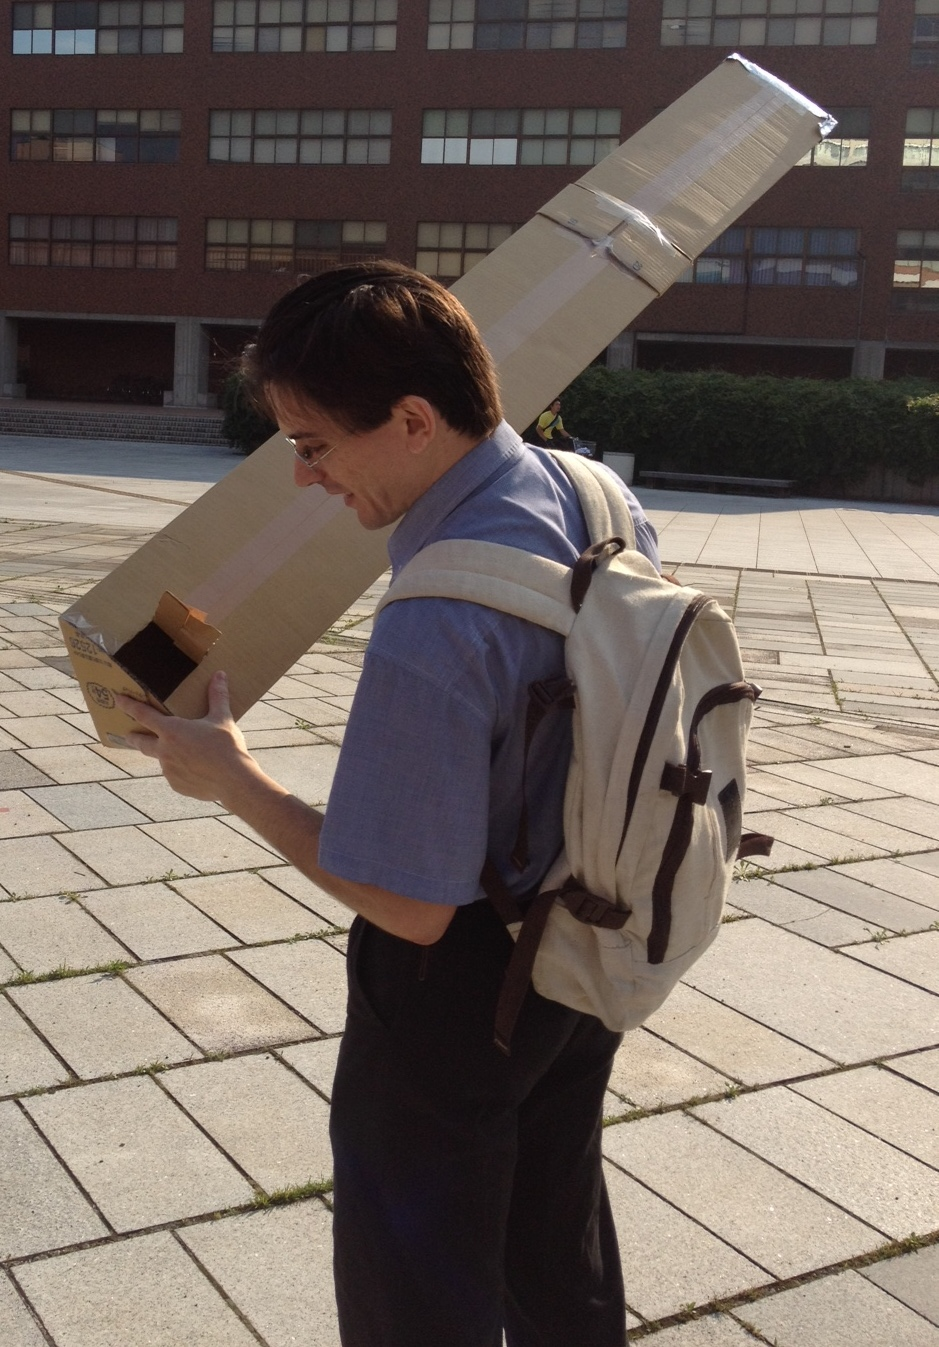
\includegraphics[width=1\textwidth]{../img/pinhole}
    \column{0.6\textwidth}
    {\small
    \begin{itemize}
      \item \structure{Name:} Claus Aranha;
      \item \structure{Country:} Brazil;
      \item \structure{Research:}
      \begin{itemize}
        \item Evolutionary Algorithms;
        \item Artificial Life;
      \end{itemize}
      \item \structure{Hobbies:}
      \begin{itemize}
        \item Programming Games;
        \item Watching Stars;
      \end{itemize}
        \medskip

      \item \structure{webpage:}\\ {\smaller \url{http://conclave.cs.tsukuba.ac.jp}}
    \end{itemize}
    }
  \end{columns}
\end{frame}

\begin{frame}
  \frametitle{What is a Programming Challenge? - 2}

  \begin{itemize}
    \item Program Challenges are good for \structure{Practicing Algorithms}
    \bigskip

    \item Program Challenges are good for \structure{Rapid Prototyping}
    \bigskip

    \item Program Challenges are used for \structure{Work Recruiting}
    \bigskip

    \item Program Challenges are also \structure{very fun puzzles!}
  \end{itemize}
\end{frame}

\begin{frame}
  \frametitle{This course is about Programming Challenges}

  The Goal of this course is \structure{solve programming challenges} to \alert{become better at programming}.

  \vfill

  We will study \structure{algorithms and techniques} that are common in
  \structure{programming competitions}
\end{frame}

\subsection{Course Outline}
\begin{frame}
  \frametitle{First Things First: Important Notices}

  \begin{block}{Manaba Page}
    All lecture notes and announcements for this course will be done
    through MANABA. Access the url below:

    \medskip

    \url{https://manaba.tsukuba.ac.jp/ct/course_1149028}\\
    Registration Code: 7255921
  \end{block}
  \begin{exampleblock}{Language}
    \begin{itemize}
      \item \structure{Lectures}: Japanese
      \item \structure{Slides and materials}: English
      \item \structure{Exercises}: English
      \item \structure{Questions, Mails and Homework}: Any language
    \end{itemize}
  \end{exampleblock}
\end{frame}



\subsection{Example of a Programming Challenge}
\begin{frame}
  \frametitle{What is a Programming Challenge? - 0}

  Consider a string with $N$ characters chosen from $G,C,T,A$. Ex:

  \begin{center}
    \emph{\alert<2>{GACA\alert<4>{CATACAG}AT}TA\alert<3>{CATTAC}AGA ... GATACCAGATA}
  \end{center}

  When you receive pair of indexes $s$ and $e$, calculate the number of "CA"s between $N_s$ and $N_e$. Ex:

  \begin{itemize}
    \item \only<2->{s = 0, e = 12\hfill 3 repetitions}
    \item \only<3->{s = 15, e = 20\hfill 1 repetition}
    \item \only<4>{s = 4, e = 10\hfill 2 repetitions}
  \end{itemize}
\end{frame}

\begin{frame}[t]
  \frametitle{What is a Programming Challenge? - 1}

  \begin{center}
    \emph{GACACATACAGATTACATTACAGA ... GATACCAGATA}
    \only<2>{\emph{000112222333333344444555 ... 88888899999}}
  \end{center}

  \begin{block}{Algorithm Idea 1}
    Start a counter $c = 0$, loop from $N_s$ to $N_e$,
    and every time you find "CA", add to the counter.
    \bigskip

    \alert{Problem: If we have many queries, can we do faster?}
  \end{block}

  \begin{onlyenv}<2>

  \begin{block}{Algorithm Idea 2}
    Creat an auxiliary array $A$, that keeps the \alert{Cummulative sum} of "CA"s from $N_0$ to $N_i$.

    \bigskip

    If we want to know the answer, we calculate $A_e - A_s$.
  \end{block}
  \end{onlyenv}
\end{frame}




\begin{frame}
  \frametitle{What is this course about?}

  You have learned many programming techniques...\\\hfill \structure{...but can you use them?}

  \begin{block}{Course Objective: Learning by Practice}
    \begin{itemize}
      {\small
    \item Every week: Solve 8 programming challenges;
    \item \structure{Choose} and \structure{implement} the {\bf best algorithm} for each problem;
    \item Be careful with \alert{max time}, and \alert{max memory};
    \item We will discuss algorithms, techniques and tricks;
      }
    \end{itemize}
  \end{block}

  \begin{exampleblock}{Course Goal:}
    Improve programming abilities, techniques and familiarity.
  \end{exampleblock}
\end{frame}

\begin{frame}
  \frametitle{Warnings about this class}
  \begin{alertblock}{1- Heavy Workload}
    \begin{itemize}
    \item Starts easy, but hard in the end;
    \item A few hours/week of homework;
    \item Lots of debugging;

      \bigskip

    \item Hint: Do your homework early!
    \end{itemize}
  \end{alertblock}

  \begin{alertblock}{2- Course Language}
    \begin{itemize}
    \item My Japanese is not very good ;-) Let's talk in C++!
    \item All the course materials are in English;
    \item You can make your homework in Japanese;

      \bigskip

    \item Practice some English in this course too! :-)
    \end{itemize}
  \end{alertblock}

\end{frame}

\section{Programming Challenges}
\subsection{Example}

\begin{frame}
  \frametitle{What is a ``Programming Challenge''?}

  A \structure{puzzle} that you solve by \structure{programming}.

  \bigskip

  Parts of a Programming Challenge:
  \begin{itemize}
  \item Description;
  \item Standard input;
  \item Standard output;
  \item Examples;
  \end{itemize}

  \bigskip

  Task: Write a program that:
  \begin{itemize}
    \item Reads the input;
    \item Prints the \structure{correct} output;
    \item And nothing else!
  \end{itemize}
\end{frame}

\subsection{Tutorial}
\begin{frame}
  \frametitle{Tutorial: ``Relational Operator'' (1)}

  All challenges are listed at the page:\\
  {\smaller \url{http://conclave.cs.tsukuba.ac.jp/lecture/monitor.html}}

  \bigskip

  Let's click on "Relational Operator"

  \begin{center}
    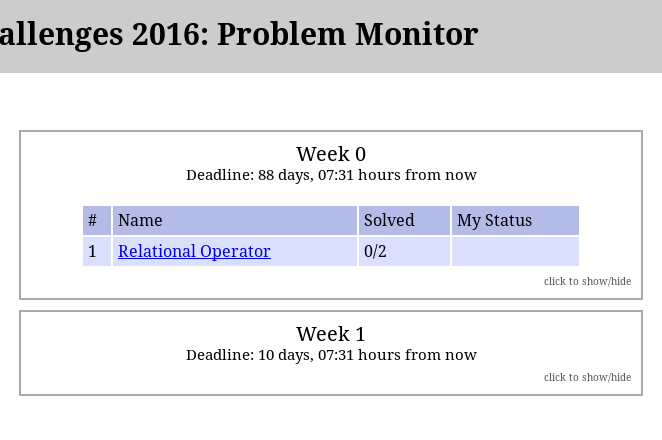
\includegraphics[width=.7\textwidth]{../img/monitorpage}
  \end{center}

\end{frame}

\begin{frame}
  \frametitle{Tutorial: ``Relational Operator'' (2)}

  The link takes you to the UVA (University of Valladolid) homepage (\alert{Please use an ad blocker!}).

  \bigskip

  Here you can see the problem description, and the links to submit the problem.

  \begin{center}
    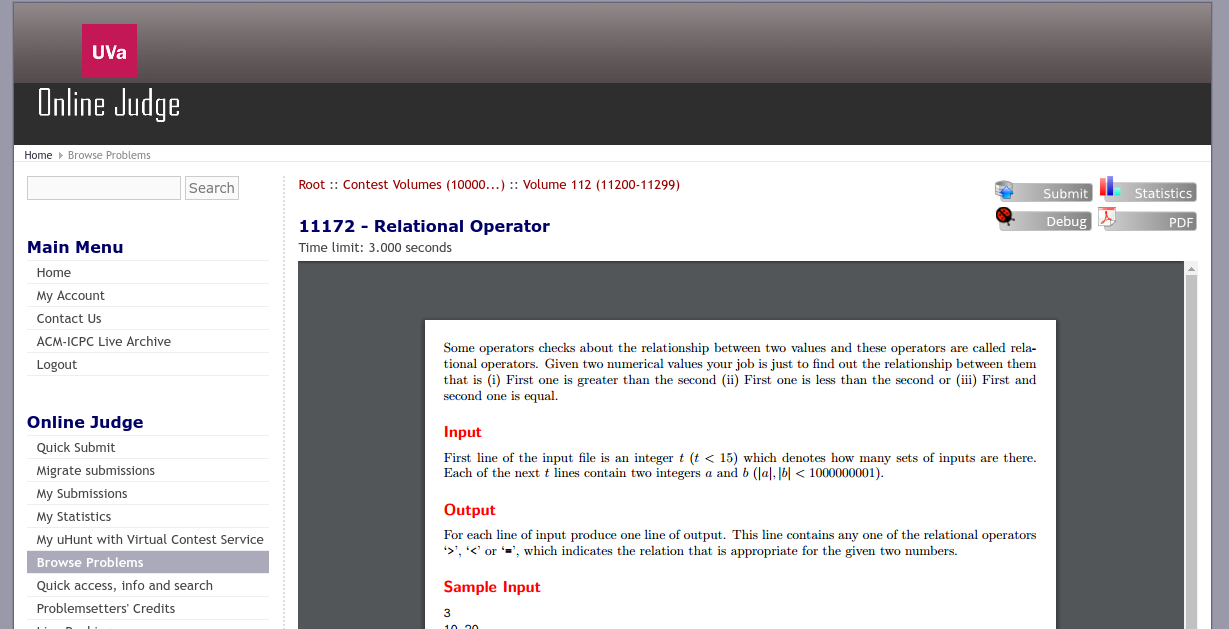
\includegraphics[width=.9\textwidth]{../img/relationaloperator}
  \end{center}
\end{frame}

\begin{frame}
  \frametitle{Tutorial: ``Relational Operator'' (3)}

  \begin{block}{Description}
    {\smaller \emph{
    Some operators checks about the relationship between two values and these
    operators are called relational operators. Given two numerical values \alert{your
    job is} just to find out the relationship between them that is (i) First one
    is greater than the second (ii) First one is less than the second or (iii)
    First and second one is equal.}}
  \end{block}

  \begin{itemize}
    \item Reading the description can be the hardest part!
    \item For this challenge, you just need to:
    \begin{itemize}
      \item If the first number is bigger than the second; print ">"
      \item If the first number is smaller than the second; print "<"
      \item If both numbers are equal, print "="
    \end{itemize}
  \end{itemize}
  Very easy!
\end{frame}


\begin{frame}
  \frametitle{Tutorial: ``Relational Operator'' (4)}

  \begin{block}{Input and Output}
    {\smaller
    \alert{Input}\\
    First line of the input file is an integer $t (t < 15)$ which denotes how many sets of inputs are there.
    Each of the next t lines contain two integers a and b (|a|, $|b| < 1000000001$).
    \medskip

    \alert{Output}\\
    For each line of input produce one line of output. This line  contains any one of the relational operators
    ''>'', ''<'' or ''='', which indicates the relation that is appropriate for the given two numbers.
  }
  \end{block}

  \begin{itemize}
    \item It is important to read the \alert{size} of the problem!
    \item Pay attention to the \alert{shape} of the output!
  \end{itemize}

\end{frame}

\begin{frame}
  \frametitle{Tutorial: ``Relational Operator'' (5)}
  \begin{block}{Examples}
  \alert{Sample Input}\\
  3\\
  10 20\\
  20 10\\
  10 10\\
  \alert{Sample Output}\\
  <\\
  >\\
  =\\
  \end{block}

  \begin{itemize}
    \item Use the samples to test/debug your program.
    \item Use your own samples too!
    \item Use the samples to \structure{understand} the challenge.
  \end{itemize}
\end{frame}



\begin{frame}[fragile]
  \frametitle{Solution: C++}

\begin{block}{}
{\smaller
\begin{verbatim}
// UVA 11172 - Relational Operator
// Test if a is bigger, smaller or equal to b

#include <iostream>
using namespace std;

int main()
{
    int n; long a, b;

    cin >> n;
    for (; n > 0; n--)
    {
        cin >> a >> b;
        if (a > b) cout << ">\n";
        if (a < b) cout << "<\n";
        if (a == b) cout << "=\n";
    }
}
\end{verbatim}}
\end{block}
\end{frame}

\begin{frame}[fragile]
  \frametitle{Solution: Python}
  \begin{block}{}
\begin{verbatim}
n = int(input())

while (n > 0):
   line = input()
   tokens = line.split()
   a,b = int(tokens[0]),int(tokens[1])

   if a > b: print(">")
   if a < b: print("<")
   if a == b: print("=")

   n -= 1
\end{verbatim}
  \end{block}

\end{frame}

\begin{frame}[fragile]
  \frametitle{Solution: Java}

  {\tiny
  \begin{block}{}
\begin{verbatim}
import java.io.*;
class Main
{
   public static void main(String args[])
   {
      BufferedReader stdin = new BufferedReader(new InputStreamReader(System.in));
      BufferedWriter stdout = new BufferedWriter(new OutputStreamWriter(System.out));
      try {
      String line;
      line = stdin.readLine();
      int n = Integer.parseInt(line);

      for (int i = 0; i < n; i++)
      {
         line = stdin.readLine();
         String[] tokens = line.split("\\s+");
         long a = Integer.parseInt(tokens[0]);
         long b = Integer.parseInt(tokens[1]);

         if (a > b)
            stdout.write(">\n");
         if (a < b)
            stdout.write("<\n");
         if (a == b)
            stdout.write("=\n");
         stdout.flush();
      }
      stdout.close();
      } catch (IOException ioe) { System.out.println("I/O Exception");}
   }
}
\end{verbatim}
  \end{block}
  }
\end{frame}

\begin{frame}
  \frametitle{Java Solution -- Keep in Mind}

  \begin{itemize}
  \item All code must be in the one file;

    \medskip

  \item The \structure{static main} method must be in \structure{Main} class.

    \medskip

  \item Do not use public classes. Even Main must be non public.

    \medskip

  \item Use Buffered I/O for faster input/output.
  \end{itemize}
\end{frame}

\subsection{Submitting Your Program}

\begin{frame}
  \frametitle{Submitting the problem to UVA}
  \begin{center}
    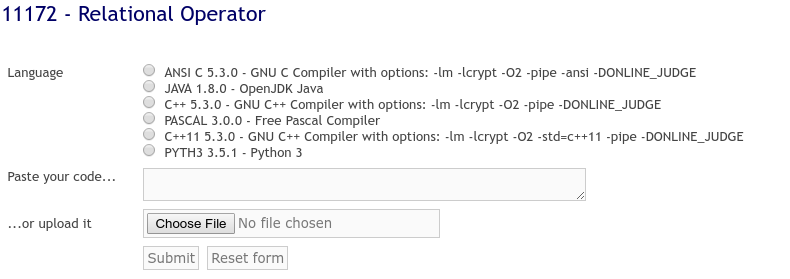
\includegraphics[width=1.1\textwidth]{../img/submitpage}
  \end{center}

  \begin{itemize}
    \item After you complete the program, use the \structure{submit} button in the UVA page;
    \item Choose your language and submit your code;
    \item You can choose C, C++, Java or Python.
  \end{itemize}
\end{frame}

\begin{frame}
  \frametitle{Submitting the problem to UVA}

    \begin{center}
      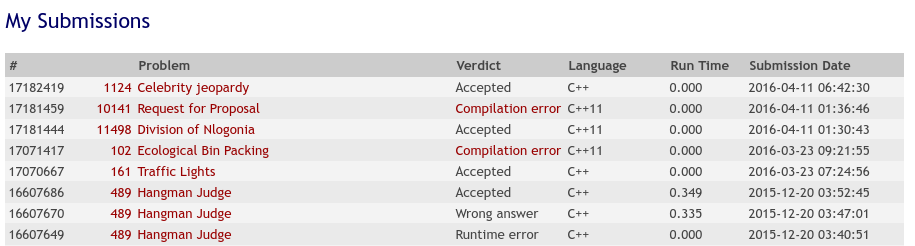
\includegraphics[width=1.1\textwidth]{../img/submissionpage}
    \end{center}

    \begin{itemize}
      \item UVA has an \structure{Automated Judge}.
      \item After 2~5 minutes, you should receive an e-mail with the result.
      \item All your results can be seen at "My Submissions" Page.
    \end{itemize}
\end{frame}

\begin{frame}
  \frametitle{Submitting the problem to UVA}

  These are the possible results:

  \bigskip

  \begin{itemize}
  \item \structure{Accepted}: Your program is correct!
    Congratulations!
  \item \structure{Presentation Error}: Small mistake in number of spaces. Congratulations!

    \bigskip

  \item \alert{Wrong Answer}: Your program is incorrect. Time to debug.

    \bigskip

  \item \alert{Time Limit Exceeded}: Your program is too slow.

  \item \alert{Memory limit exceeded}: Your program uses too much memory.

    \bigskip
  \item \alert{Runtime Error}: Your program crashed (segmentation fault!)

    \bigskip
  \end{itemize}

\end{frame}

\begin{frame}
  \frametitle{Problem Monitor Page}


  \begin{center}
    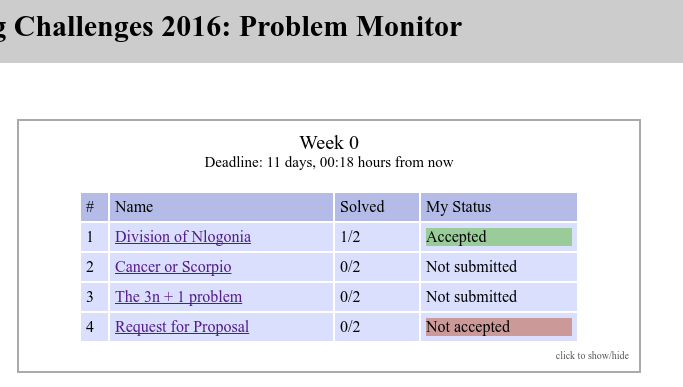
\includegraphics[width=1\textwidth]{../img/monitorpage2}
  \end{center}

  \begin{itemize}
    \item All Problems and results;
    \item All Deadlines;
  \end{itemize}

\end{frame}

\subsection{Manaba Submission}
\begin{frame}
  \frametitle{Submitting the problem to MANABA}

  {\small
  After you finish the problems listed in the monitor, you need to
  submit your source code and a comment file as a zip package to MANABA.}

  \medskip

  {\small
  \begin{columns}
    \column{0.3\textwidth}
    \column{0.4\textwidth}
    \begin{block}{s2015XXXXXX-weekYY.zip}
      \begin{itemize}
      \item problem1.cpp
      \item problem2.cpp
      \item problem5.cpp
      \item kaisetsu.txt
      \end{itemize}
    \end{block}
    \column{0.3\textwidth}
  \end{columns}
  }

  \medskip

  \begin{alertblock}{Attention}
  Submission to the UVA judge without a submission to MANABA will not
  be accepted!
  \end{alertblock}
\end{frame}

\section{Course Rules}
\subsection{Course Structure}

\begin{frame}
    \frametitle{Course Rules}

    \begin{block}{Two classes per week}
        \begin{itemize}
        \item Each week has a theme (Graphs, Maths, etc...)
        \item Friday Class: Introduction
        \item Monday Class: Problem Solving and Q\&A
        \end{itemize}
    \end{block}

    \begin{block}{Solving Problems}
        \begin{itemize}
        \item Every week there are 8 programming assignments;
        \item Deadline is Thursday 23:59
        \begin{itemize}
          \item UVA Submission
          \item MANABA Submission
        \end{itemize}
        \end{itemize}
    \end{block}
\end{frame}

\begin{frame}
  \frametitle{Outline}
  \begin{center}
    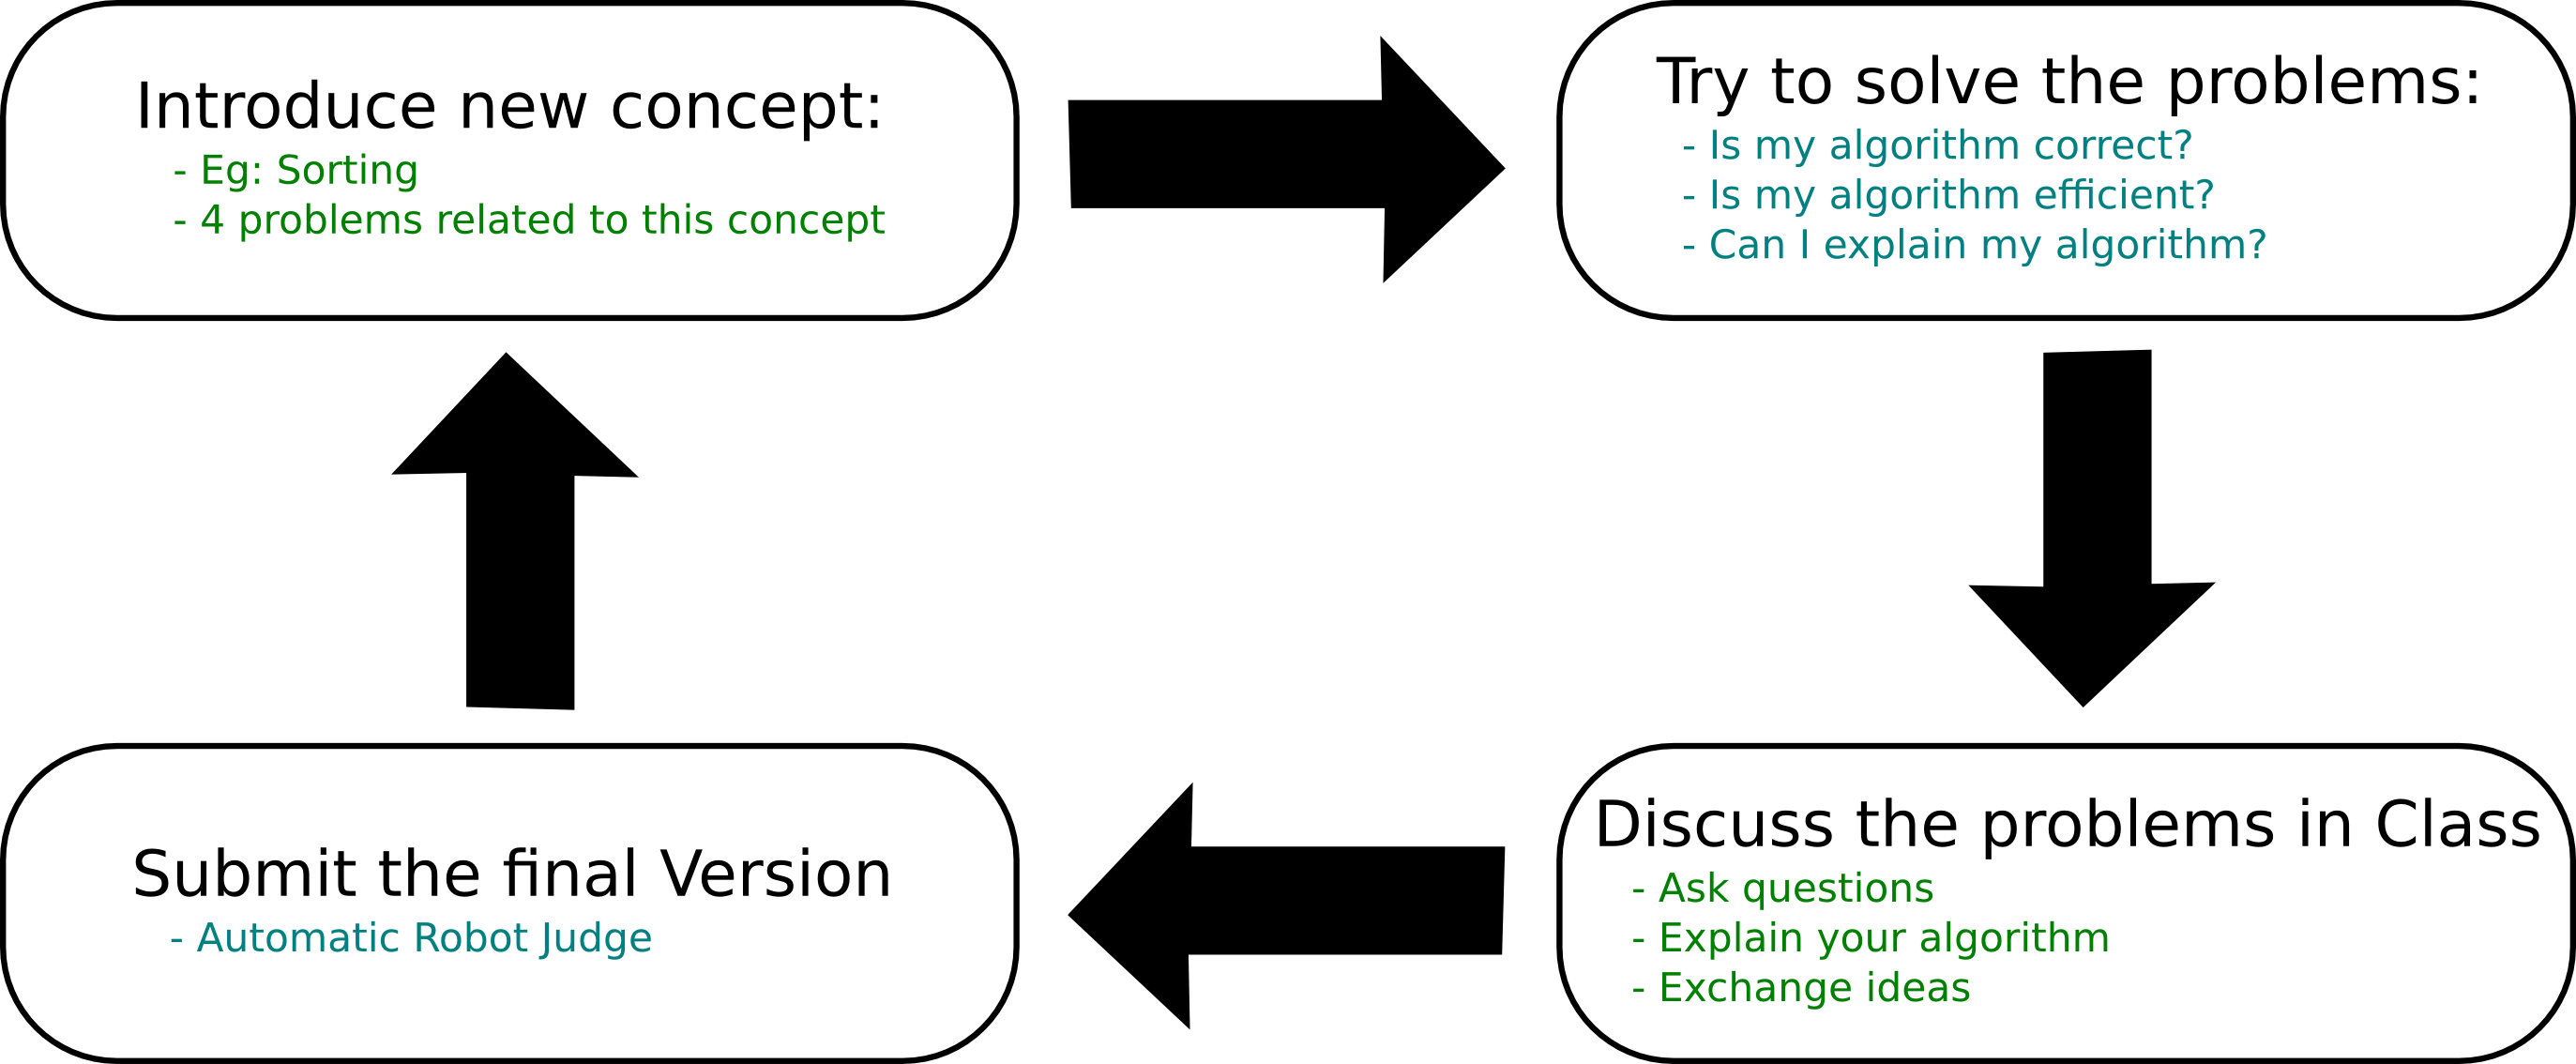
\includegraphics[width=1\textwidth]{../img/classoutline}
  \end{center}
\end{frame}

\subsection{Grading}

\begin{frame}
  \frametitle{Grading Algorithm}

  Your Grade: {\bf Base Grade} \structure{+Bonus} \alert{-Penalty}

  \begin{itemize}
    \item {\bf Base Grade}:
    \begin{itemize}
      \item You solved 2/8 problem/week: "C"
      \item You solved 3/8 problems/week: "B"
      \item You solved 4/8 problems/week: "A"
    \end{itemize}

    \bigskip

    \item \structure{+Bonus}
    \begin{itemize}
      \item 5\% of best student in each category.
      \item Special collaboration to the class.
    \end{itemize}

    \bigskip
    \item \alert{-Penalty}
    \begin{itemize}
      \item More than 25\% of homework submitted late.
    \end{itemize}
  \end{itemize}


\end{frame}

\begin{frame}[fragile]
  \frametitle{Evaluating and Grading: KAISETSU file}

  \begin{itemize}
    \item Submit a TEXT (not word) file with your impressions of the problems, class, life, together with your code.
    \item Kaisetsu file can be in any Japanese or English.
  \end{itemize}

  \bigskip

  \begin{exampleblock}{Example}
    {\smaller
\begin{verbatim}
Name: Claus, ID: 98884735
# Problem 1:
This problem was very easy, but I did a stupid mistake
and it took me three hours to solve. I found the solution
when I tried a new test case.

# Problem 2:
This problem was very hard, and I was very hungry, so I
gave up.
\end{verbatim}}
  \end{exampleblock}

\end{frame}

\begin{frame}
  \frametitle{Evaluation and Grading (5) -- about plagiarism}

  The assignments are \alert{individual}. Use your \structure{own
    strength} to solve the programs.

  \begin{exampleblock}{GOOD}
    \begin{itemize}
    \item Ask for ideas to your friends;
    \item Ask for ideas in the MANABA forum;
    \item Ask for help with a bug;
    \end{itemize}
  \end{exampleblock}

  \begin{alertblock}{BAD}
    \begin{itemize}
    \item Copy a solution from the internet;
    \item Copy a solution from your friends;
    \item Give your code to a friend;
    \end{itemize}
  \end{alertblock}

  Plagiarism will result in course failure, and possibly worse.
\end{frame}

\section{Resources}
\subsection{Resources}

% Class Links
\begin{frame}
  \frametitle{Useful Links}
  \begin{itemize}
  \item
    \href{https://manaba.tsukuba.ac.jp/ct/course_1149028}
         {\structure{\underline{Manaba Page}}}: All the class material
         will be here. Access Code is: 7255921

    \medskip

  \item \href{https://uva.onlinejudge.org/}{\structure{\underline{UVA Online Judge}}}:
    Use this page to submit your problems. \alert{Make an account and list the username on MANABA}

    \medskip

  \item \href{https://conclave.cs.tsukuba.ac.jp/lecture/monitor.html}{\structure{\underline{Problem Monitor}}}:
    Use this page to check deadlines and weekly problems.

    \medskip

  \item
    \href{https://www.github.com/caranha/ProgrammingChallengesLectureNotes}{\structure{\underline{Github
          Repository}}}:
    Working directory for lecture notes. Send me PR, issues!

    \medskip

  \item
    \href{https://www.udebug.com/}{\structure{\underline{uDebug}}}:
    Web service that generates test inputs and test outputs for UVA
    problems. Useful tool for this course.
  \end{itemize}
\end{frame}


% Books
% TODO: Add japanese books % Needs CJK package (or book images)
\begin{frame}
  \frametitle{Course Book}

  \begin{itemize}
  \item Competitive Programming, 3rd Edition
    (\href{http://cpbook.net/}{http://cpbook.net})

    \bigskip

  \item For suggestions of books in Japanese, please check the Manaba materials!
  \end{itemize}
\end{frame}

% udebug
\begin{frame}
  \frametitle{uDebug Tool}

  uDebug generates outputs for many different debugs. It can help you check why your program is wrong.

  \bigskip

  \url{https://www.udebug.com/}

  \bigskip

  \begin{center}
    
\includegraphics[width=0.7\textwidth]{../img/udebug}
  \end{center}
\end{frame}

% % Cat stream
% \begin{frame}
%   \frametitle{If you are still having problems...}
%
%   Watch a cat stream to relax!
%
%   \bigskip
%
%   \begin{center}
%     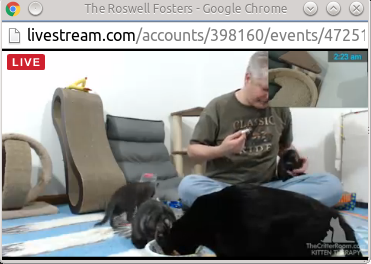
\includegraphics[width=.6\textwidth]{../img/catstream}
%   \end{center}
%
%   \bigskip
%
%   \url{http://livestream.com/FosterKittenCam/}
% \end{frame}


% Contact the professor (e-mail, twitter, webpage, room)
\begin{frame}
  \frametitle{Contact the professor}
  \begin{itemize}
  \item \structure{e-mail}: caranha@cs.tsukuba.ac.jp
  \item \structure{website}: \url{http://conclave.cs.tsukuba.ac.jp}
  %\item \structure{twitter}: @caranha

    \bigskip

  \item \structure{Room}: SB1012 -- Send an e-mail and we can talk!\\
  \end{itemize}

  \bigskip

  Both English and Japanese are okay!
\end{frame}


% Do we still have time? Fill out the forms!
% Do we still have time? Ask me questions!

\begin{frame}
  \frametitle{What to do this weekend?}

  \begin{itemize}
  \item Create an account on UVA (if you already have an account, you can use that)

    \bigskip

  \item Submit your account name to the MANABA

    \bigskip

  \item Ask any other questions you want to know!
  \end{itemize}
\end{frame}

\begin{frame}
  \frametitle{Participate in ICPC!}
  \begin{columns}
    \column{0.5\textwidth}
  \begin{itemize}
    \item Fun challenges to choose the world champion!
    \item Teams of 3 people!
    \item Registration Deadline Early of June!
  \end{itemize}

  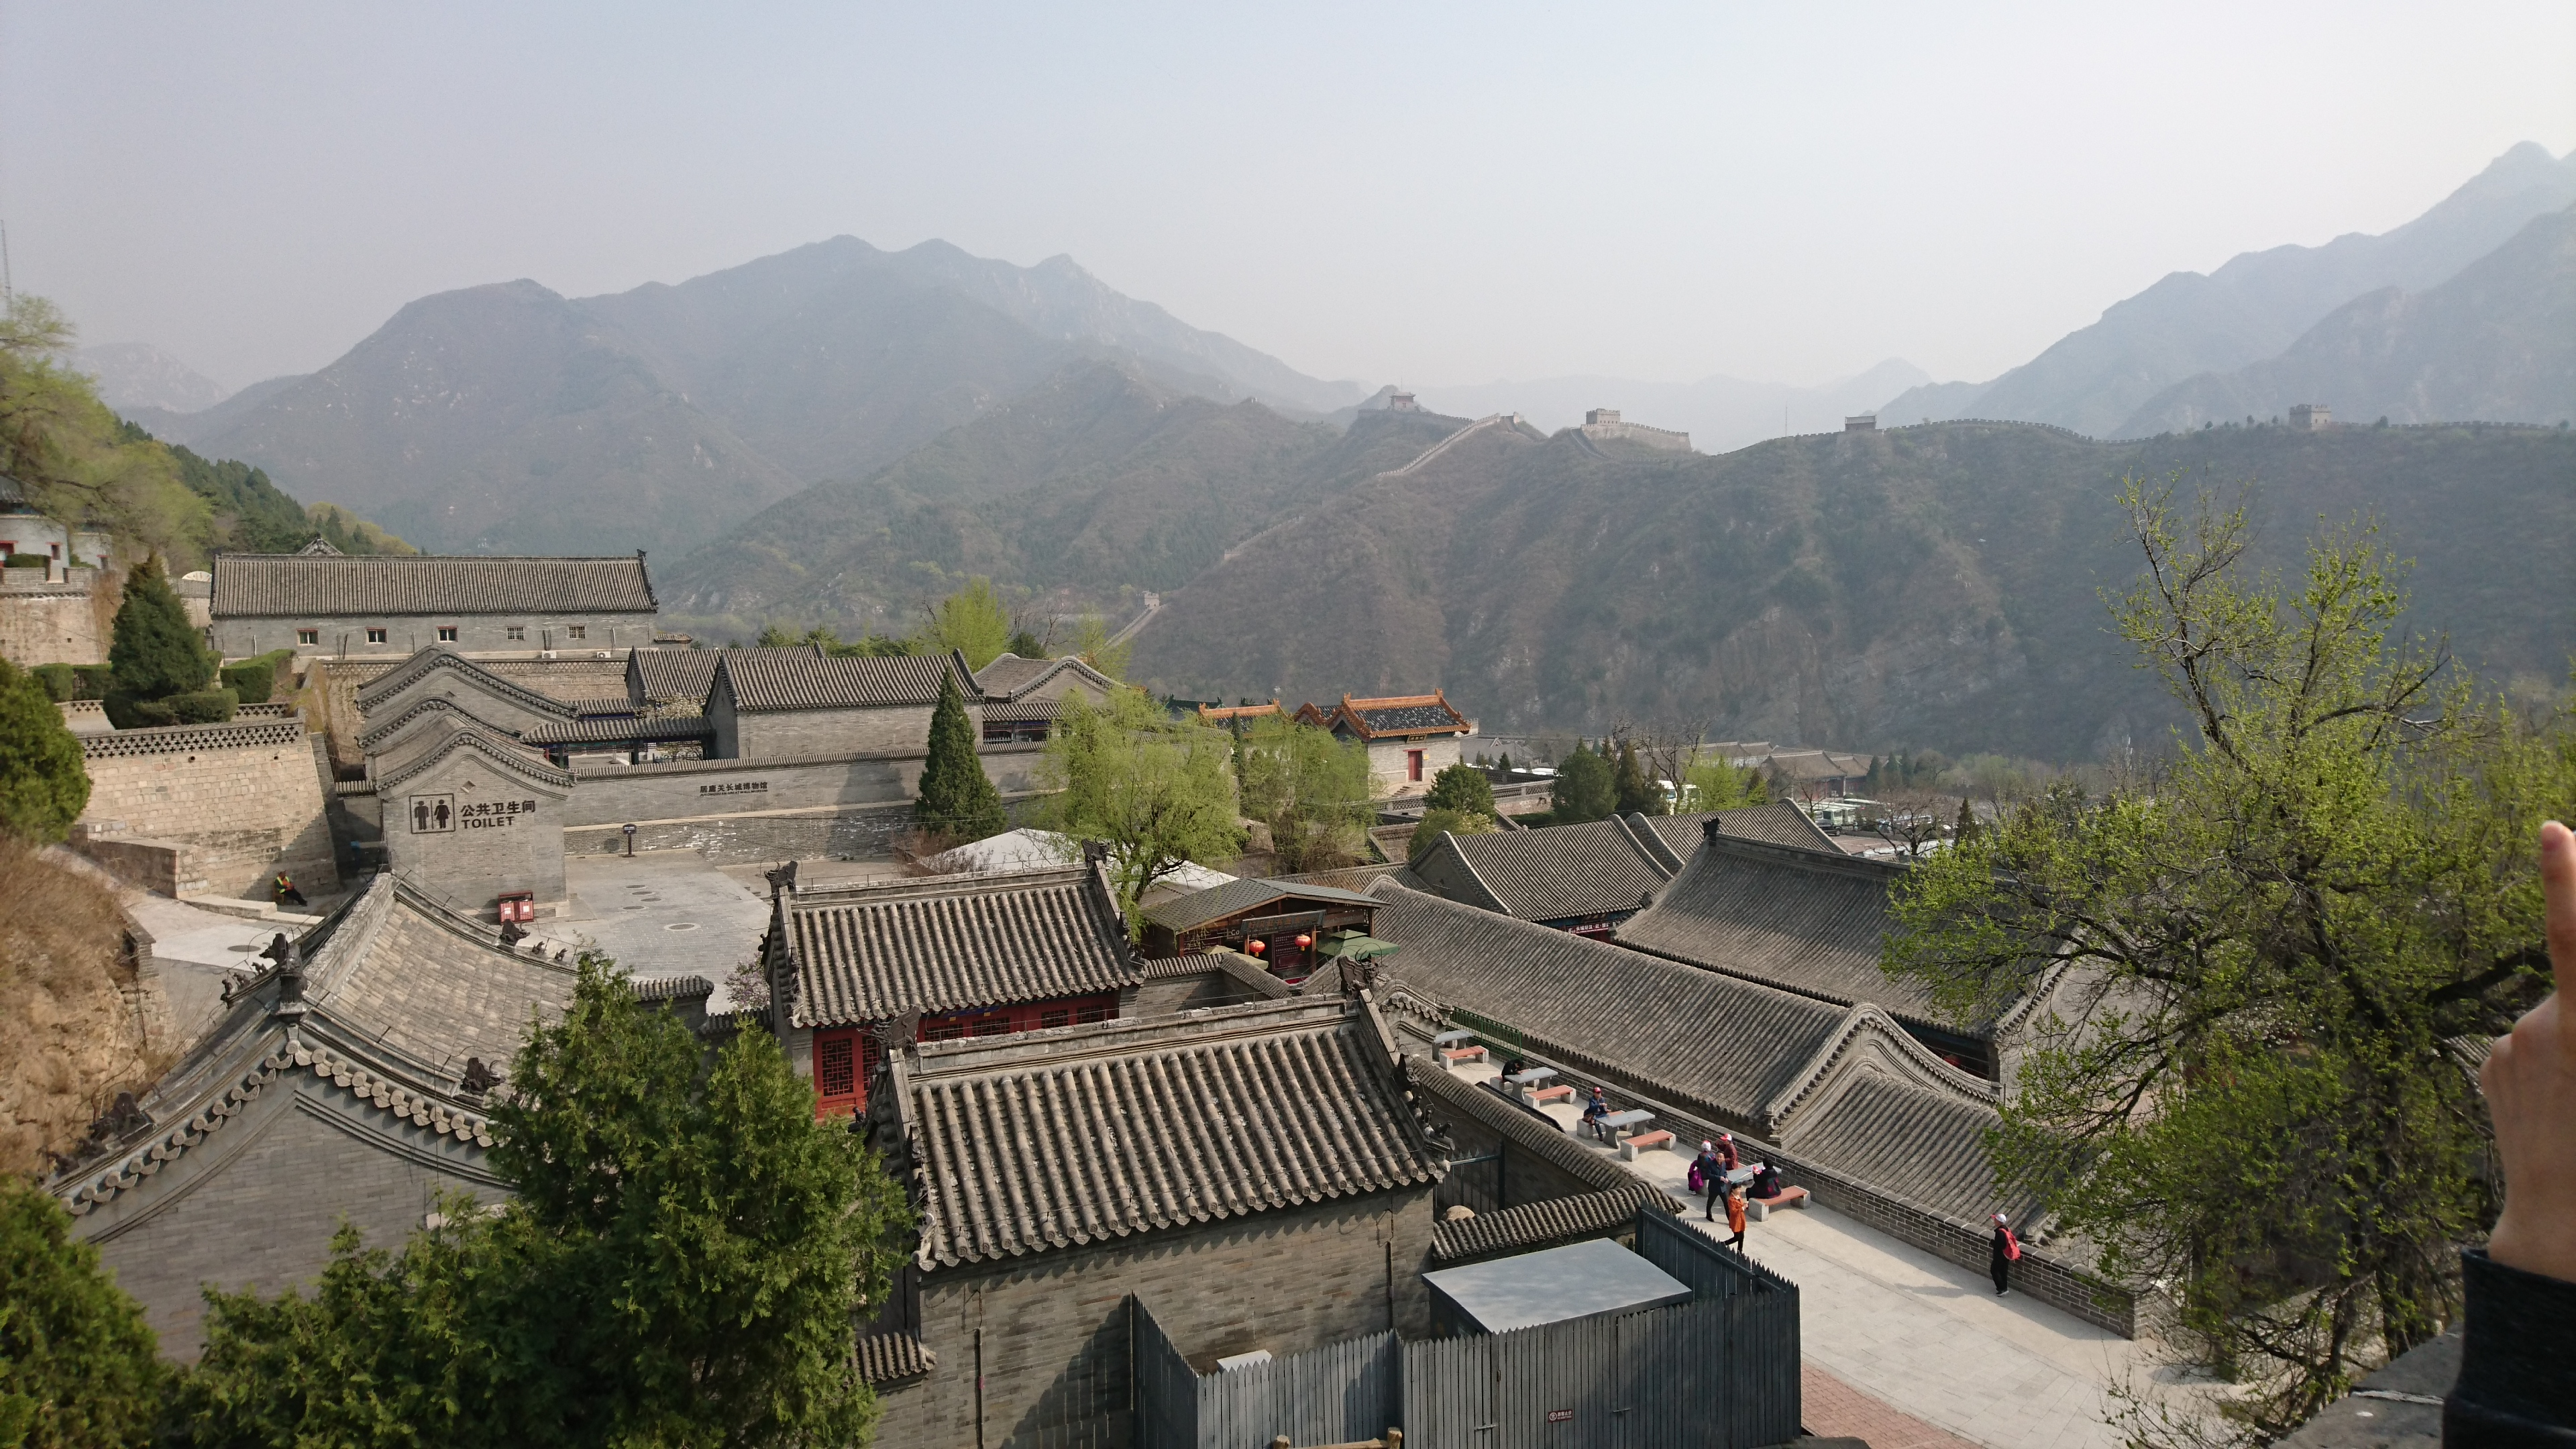
\includegraphics[width=1\textwidth]{icpc/DSC_0171}
  \column{0.5\textwidth}
  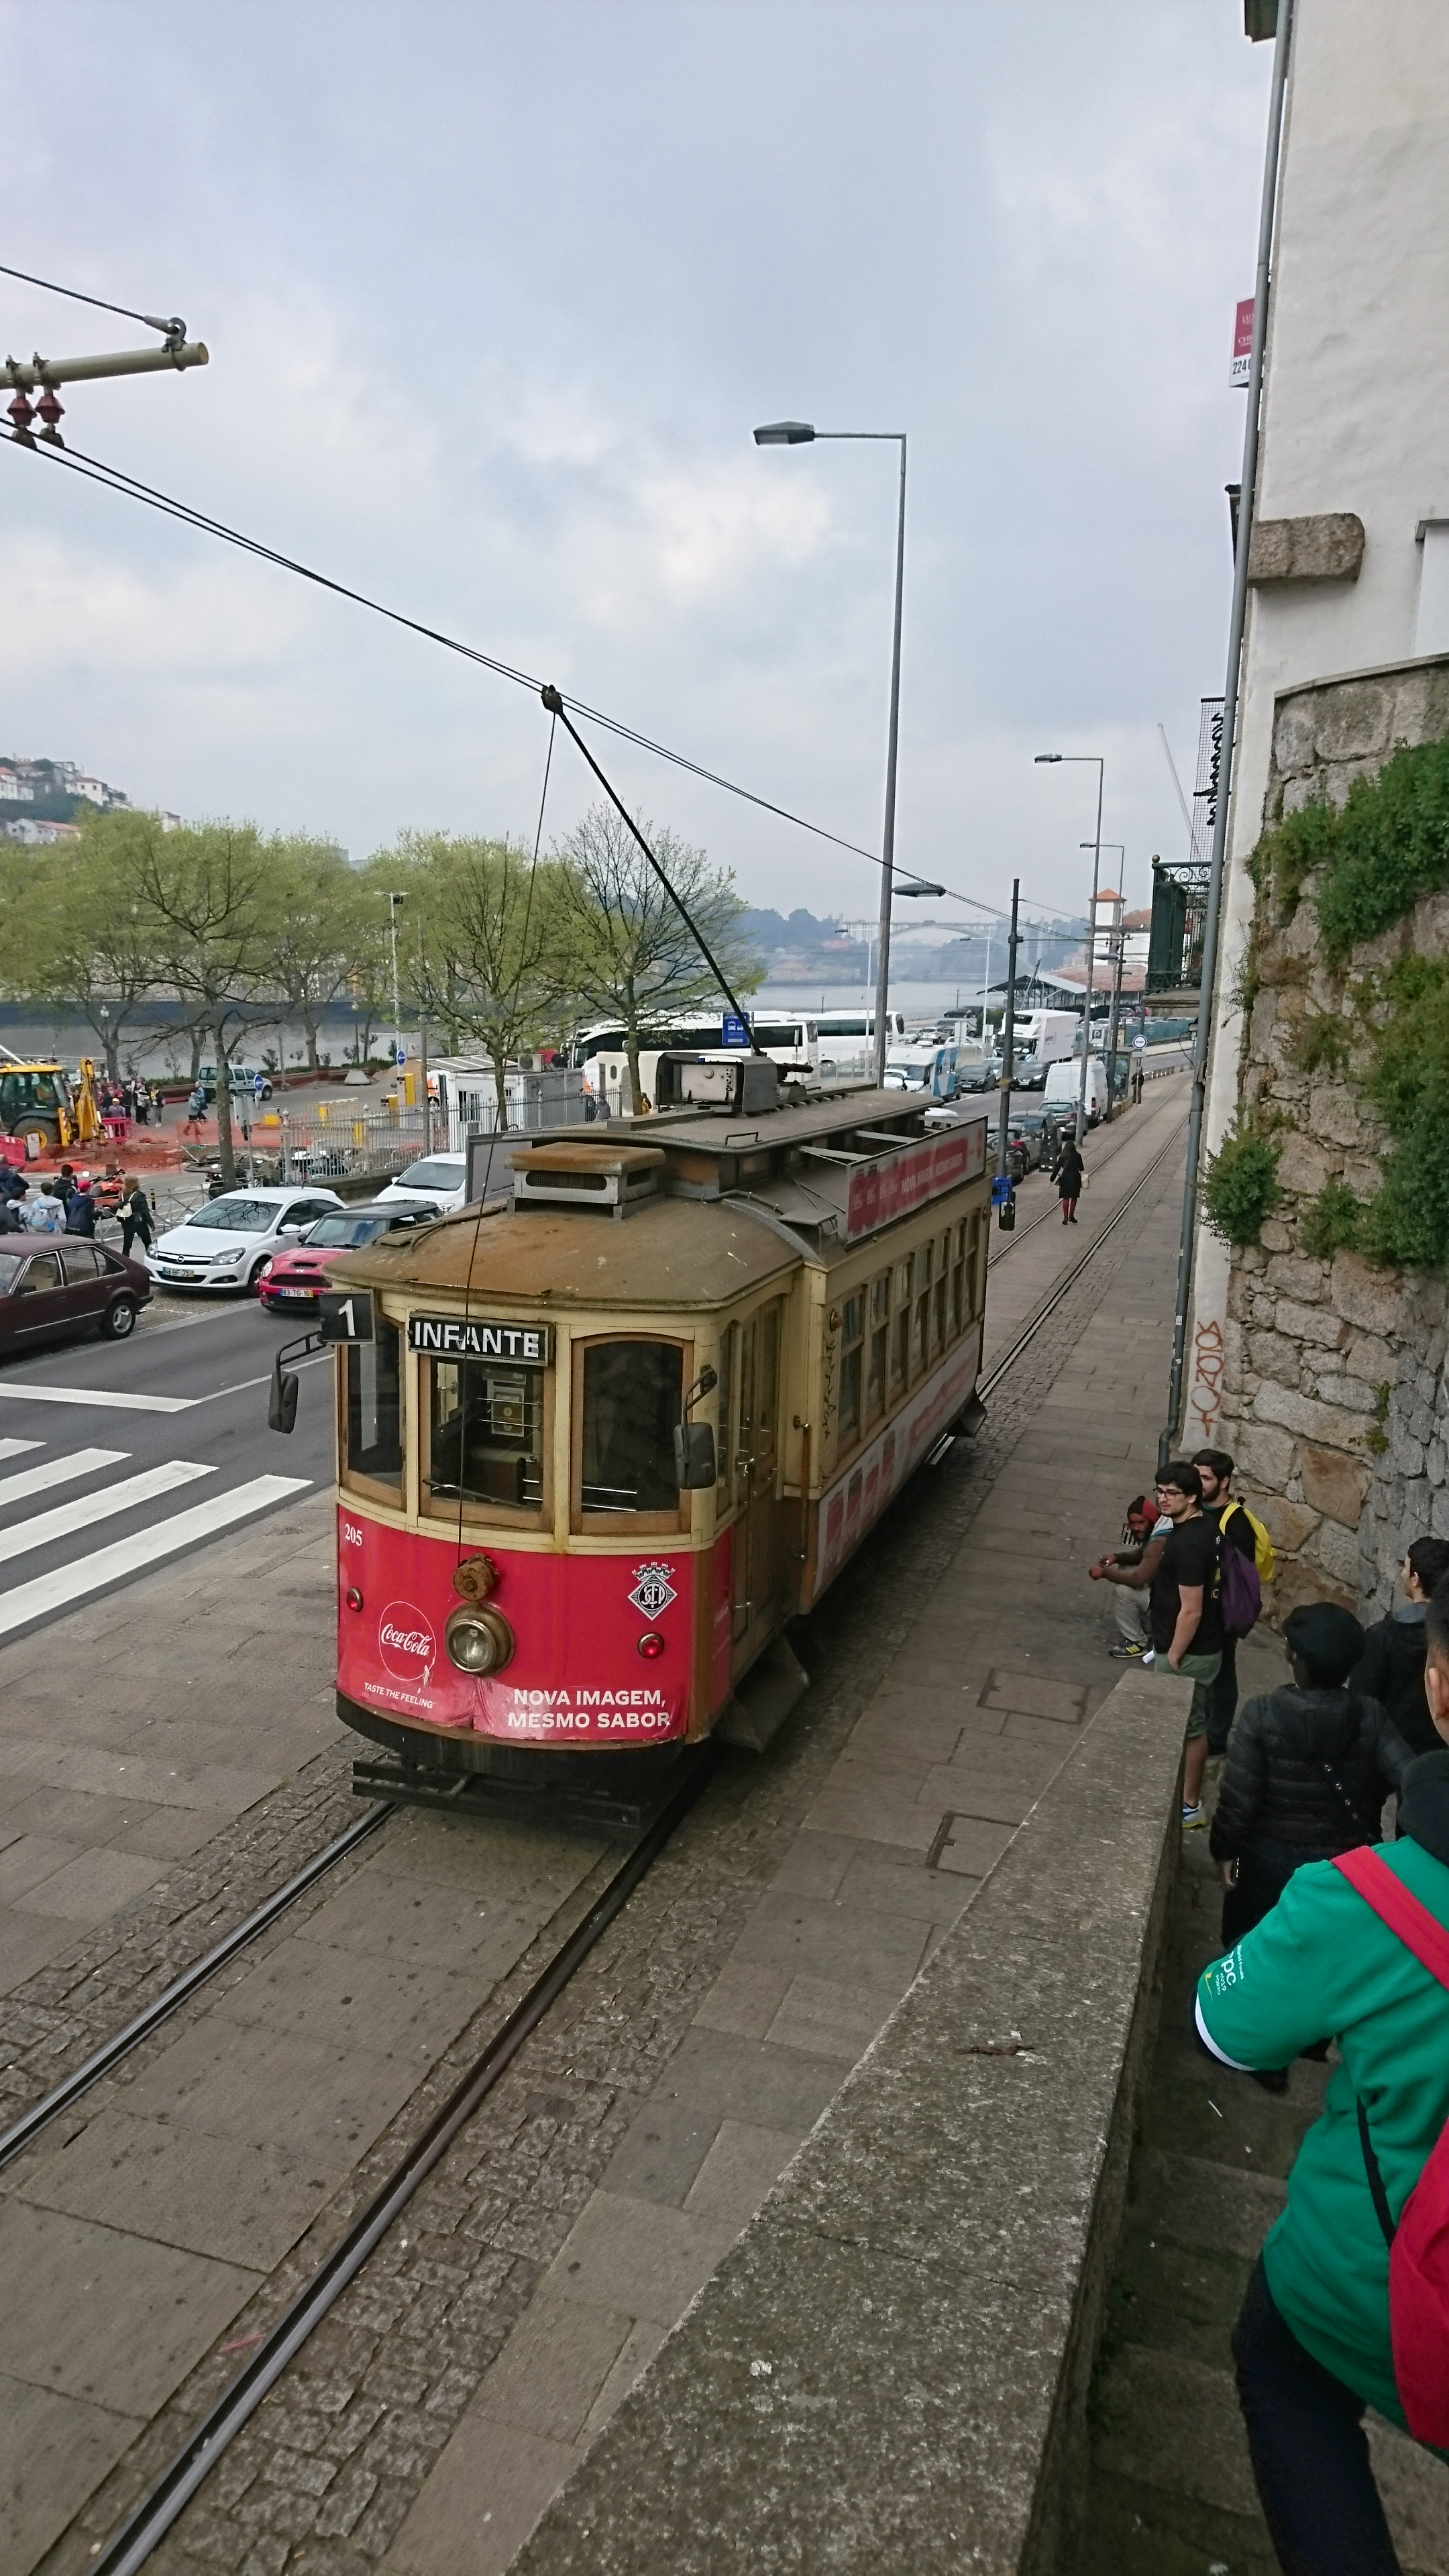
\includegraphics[width=1\textwidth]{icpc/DSC_0677}
\end{columns}
\end{frame}



\section{AdHoc Problems}
\begin{frame}
  \frametitle{Today's Class: Ad Hoc Problems}

  \begin{itemize}
  \item \structure{Ad Hoc}: Problems that don't have a single algorithm;
  \bigskip

  \item Common forms of Input and Output
  \bigskip

  \item Debugging and Creating Test Cases
  \bigskip

  \item Some Problem Analysis
  \end{itemize}

\end{frame}

\section{Problem Analysis: 3n+1}
\subsection{Wrong Answer}
\begin{frame}[fragile]
  \frametitle{Reading the Problem: 3n+1}

  \begin{block}{}
    For any two numbers $i$ and $j$, calculate the \structure{Maximum Cycle Length}.
  \end{block}

  \bigskip

\begin{verbatim}
Algorithm A(n)
1. print n
2. if n == 1 then STOP
3. if n is odd then n = 3n + 1
4. else n = n/2
5. GOTO 2


Example: A(22)
22 11 34 17 52 26 13 40 20 10 5 16 8 4 2 1

Size: 16
\end{verbatim}
\end{frame}

\begin{frame}[fragile]
  \frametitle{Problem 3n+1 -- Solution 1}
\begin{verbatim}
while true:
  try:
    line = input()
    max = 0
    tk = line.split()
    i, j = int(tk[0]), int(tk[1])
    for n in range(i, j+1):
      count = 1
      while n != 1:
        if n % 2 == 1: x = 3 * x + 1
        else: n = n / 2
        count += 1
      if count > max: max = count
      print (line, max)
  except EOFError: break
\end{verbatim}
\end{frame}

\begin{frame}
  \frametitle{Solution 1: Problem!}

  \begin{itemize}
    \item Solution 1 solves all \structure{Sample Input} correctly.
    \bigskip

    \item But we still get \alert{Wrong Answer!}
    \bigskip

    \item Why??? :-(
  \end{itemize}
\end{frame}

\begin{frame}[fragile]
  \frametitle{Solution 1: Traps!}

  \begin{itemize}
    \item Solution 1 solves all \structure{Sample Input} correctly.
    \bigskip

    \item If we try the input: \alert{20 10} -- output is \alert{nothing!}
\begin{verbatim}
for x in range(i, j+1):   <-- Error is here!
  ...
  print (line, max)
\end{verbatim}
    \bigskip

    \item The sample input has \alert{no examples} with "\alert{$i > j$}"!
  \end{itemize}
\end{frame}

\begin{frame}
  \frametitle{Solution 1: Traps!}

    \begin{block}{Input Description}
    The input will consist of a series of \alert{pairs of integers} i and j, one pair of
    integers per line. All integers will be \alert{less than 10,000 and greater than 0.}

    \bigskip

    You should process all pairs of integers and for each pair determine the maximum
    cycle length over \alert{all integers between and including i and j}.

    \bigskip

    You can \alert{assume that no operation overflows a 32-bit integer}.
    \end{block}
    \bigskip

    The only rules are those \structure{expressely written!}
\end{frame}

\begin{frame}
  \frametitle{Solution 1: Traps!!!!!}

  \begin{itemize}
    \item First rule of Programming Challenges: \\ \hspace{1cm}\alert{Assume Worst Case}
    \item Always try the worst case input!

    \bigskip

    \begin{itemize}
      \item Number is Negative; Number is zero;
      \item Number is out of order (or in order);
      \item Number is repeated;
      \smallskip

      \item Graph is unconnected; Graph is Fully connected;
      \item Lines are parallel; Points are in the same place;
      \item Area is 0; Angle is 0;
      \smallskip

      \item Input is very long;
      \item Input is very short;
    \end{itemize}
    \bigskip

    \item If it is not against the rules: \alert{It will happen!}
    \item This also happens in programs in the real world.
  \end{itemize}
\end{frame}

\subsection{Time Limited Exceeded}

\begin{frame}[fragile]
  \frametitle{Problem 3n+1 -- Solution 2}
\begin{verbatim}
while true:
  try:
    line = input()
    max = 0
    tk = line.split()
    i, j = int(tk[0]), int(tk[1])
    for n in range(min(i, j), max(i, j)+1): # FIXED!
      count = 0
      while n != 1:
        if n % 2 == 1: n = 3 * n + 1
        else: n = n / 2
        count += 1
      if count > max: max = count
      print (line, max)
  except EOFError: break
\end{verbatim}
\end{frame}

\begin{frame}
  \frametitle{Solution 2: Time Limited Exceeded!}
  \begin{itemize}
    \item All the inputs are correct.
    \bigskip

    \item But now we have \alert{Time Limited Exceeded}
    \bigskip

    \item Why?
  \end{itemize}
\end{frame}

\begin{frame}[fragile]
  \frametitle{Solution 2: Cost Calculation}

    \begin{block}{Input Description}
    All integers will be \alert{less than 10,000 and greater than 0.}
    \bigskip

    You can \alert{assume that no operation overflows a 32-bit integer}.
    \end{block}
    \bigskip

    \begin{itemize}
      \item What happens when the input is \structure{1 10000}?
\begin{verbatim}
1 10000 262
\end{verbatim}
      \bigskip

      \item The longest sequence in 1, 10000 has 262 steps.
      \item But we calculate \alert{all} sequences between 1, 10000.
      \item Worst case: 10000*262 = 2,000,000 steps!
      \bigskip

      \item For only one query!
    \end{itemize}
\end{frame}

\begin{frame}[fragile]
  \frametitle{Solution 2: Memoization}

  \begin{itemize}
    \item Let's think about A();
\begin{verbatim}
A(22):  22 11 34 17 52 26 13 40 20 10 5 16 8 4 2 1
A(11):  11 34 17 52 26 13 40 20 10 5 16 8 4 2 1
A(17):  17 52 26 13 40 20 10 5 16 8 4 2 1
A(13):  13 40 20 10 5 16 8 4 2 1
A(10):  10 5 16 8 4 2 1
A(8) :  8 4 2 1
\end{verbatim}
    \bigskip

    \item Do we need to \alert{Recalculate} every time we see a new number?
  \end{itemize}

  \begin{block}{Good Technique: Memoization}
    If we know that we will use a result again in the future,
    we should \alert{store this result in the memory}.
  \end{block}
\end{frame}

\begin{frame}[fragile]
  \frametitle{Solution 2: Memoization Idea}
\begin{verbatim}
  table = {}
  table[1] = 1

  def A(n):
    if n in table.keys():
      return table[n]
    else:
      if n % 2 == 1:
        table[n] = 1 + A(3*n + 1)
      else:
        table[n] = 1 + A(n/2)
    return table[n]
\end{verbatim}
\end{frame}

\section{How to Solve Problems}
\subsection{Programming Challenge Workflow}
\begin{frame}
  \frametitle{A Programming Challenge Workflow}

  \begin{center}
    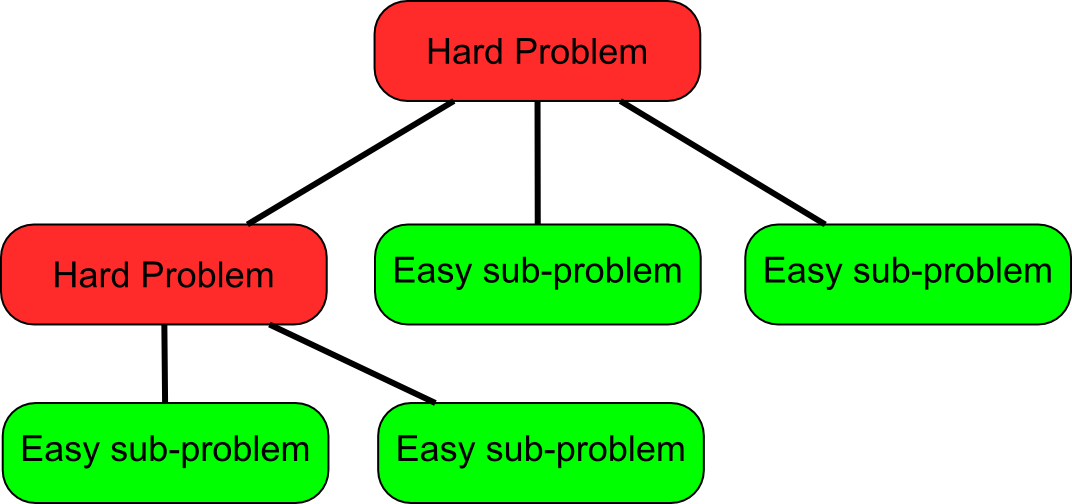
\includegraphics[width=0.5\textwidth]{../img/breakingtheproblem}
  \end{center}

  Trick to solve problems without bugs: Break the problem down
  \bigskip

  \begin{itemize}
  \item How to calculate the function $A()$;
  \item Imagine the worst possible cases ($i > j$);
  \item Calculate cost of solution;
  \item Improve speed with memoization;
  \end{itemize}
\end{frame}

\subsection{Programming Challenge Workflow}
\begin{frame}
  \frametitle{A Programming Challenge Workflow}

  Common Steps for Programming challenges:
  \bigskip

  \begin{itemize}
  \item Task 1: Read the problem description;
  \item Task 2: Read the input/output;
  \item Task 3: Think about the algorithm;
  \item Task 4: Write the Code;
  \item Task 5: Test the program on example data;
  \item Task 6: Test the program on hidden data;
  \end{itemize}
\end{frame}


\subsection{Task 1: Reading The Problem}
\begin{frame}
  \frametitle{Task 1: Understanding the Problem Description}

  The English description is so hard!

  \bigskip

  \begin{block}{Don't Worry:}
  \begin{enumerate}
  \item Separate the text into \structure{flavor} and \structure{rules};
  \item Sometimes it is easy to read the input/output first, and then
    the text;
  \item Problems with a lot of \structure{flavor} are usually not very hard.;
  \end{enumerate}
  \end{block}
\end{frame}

\begin{frame}
  \frametitle{Example: Problem 11559 -- Event Planning}

  {\smaller
  \begin{alertblock}{Flavor:}
    As you didn't show up to the yearly general meeting of the Nordic
    Club of Pin Collectors, you were unanimously elected to organize
    this years excursion to Pin City.  You are free to choose from a
    number of weekends this autumn, and have to find a suitable hotel
    to stay at, preferably as cheap as possible.
  \end{alertblock}

  \begin{exampleblock}{rules}
    You have some \structure{\underline{constraints}}: The total
    \structure{\underline{cost}} of the trip must be within
    \structure{\underline{budget}}, of course. All participants
    \structure{\underline{must}} stay at the same hotel, to avoid last years
    catastrophe, where some members got lost in the city, never being seen
    again.
  \end{exampleblock}}

  \bigskip

  {\bf Keywords:} constraints, minimum, maximum, cost, rules, number,
  etc...
\end{frame}

\begin{frame}
  \frametitle{Hints for hard to read problems}

  \begin{columns}
    \column{0.7\textwidth}
    {\small
    \begin{itemize}
    \item First, look at the \structure{sample input and output};
    \item Write the idea of the problem on paper
    \item Use the Paper: mark keywords;
    \item Use the Paper: cut flavor;
    \item \alert{Read the problem again!};
    \item \alert{Do not begin programming until you understand the problem!}
    \end{itemize}
    }
    \column{0.3\textwidth}
    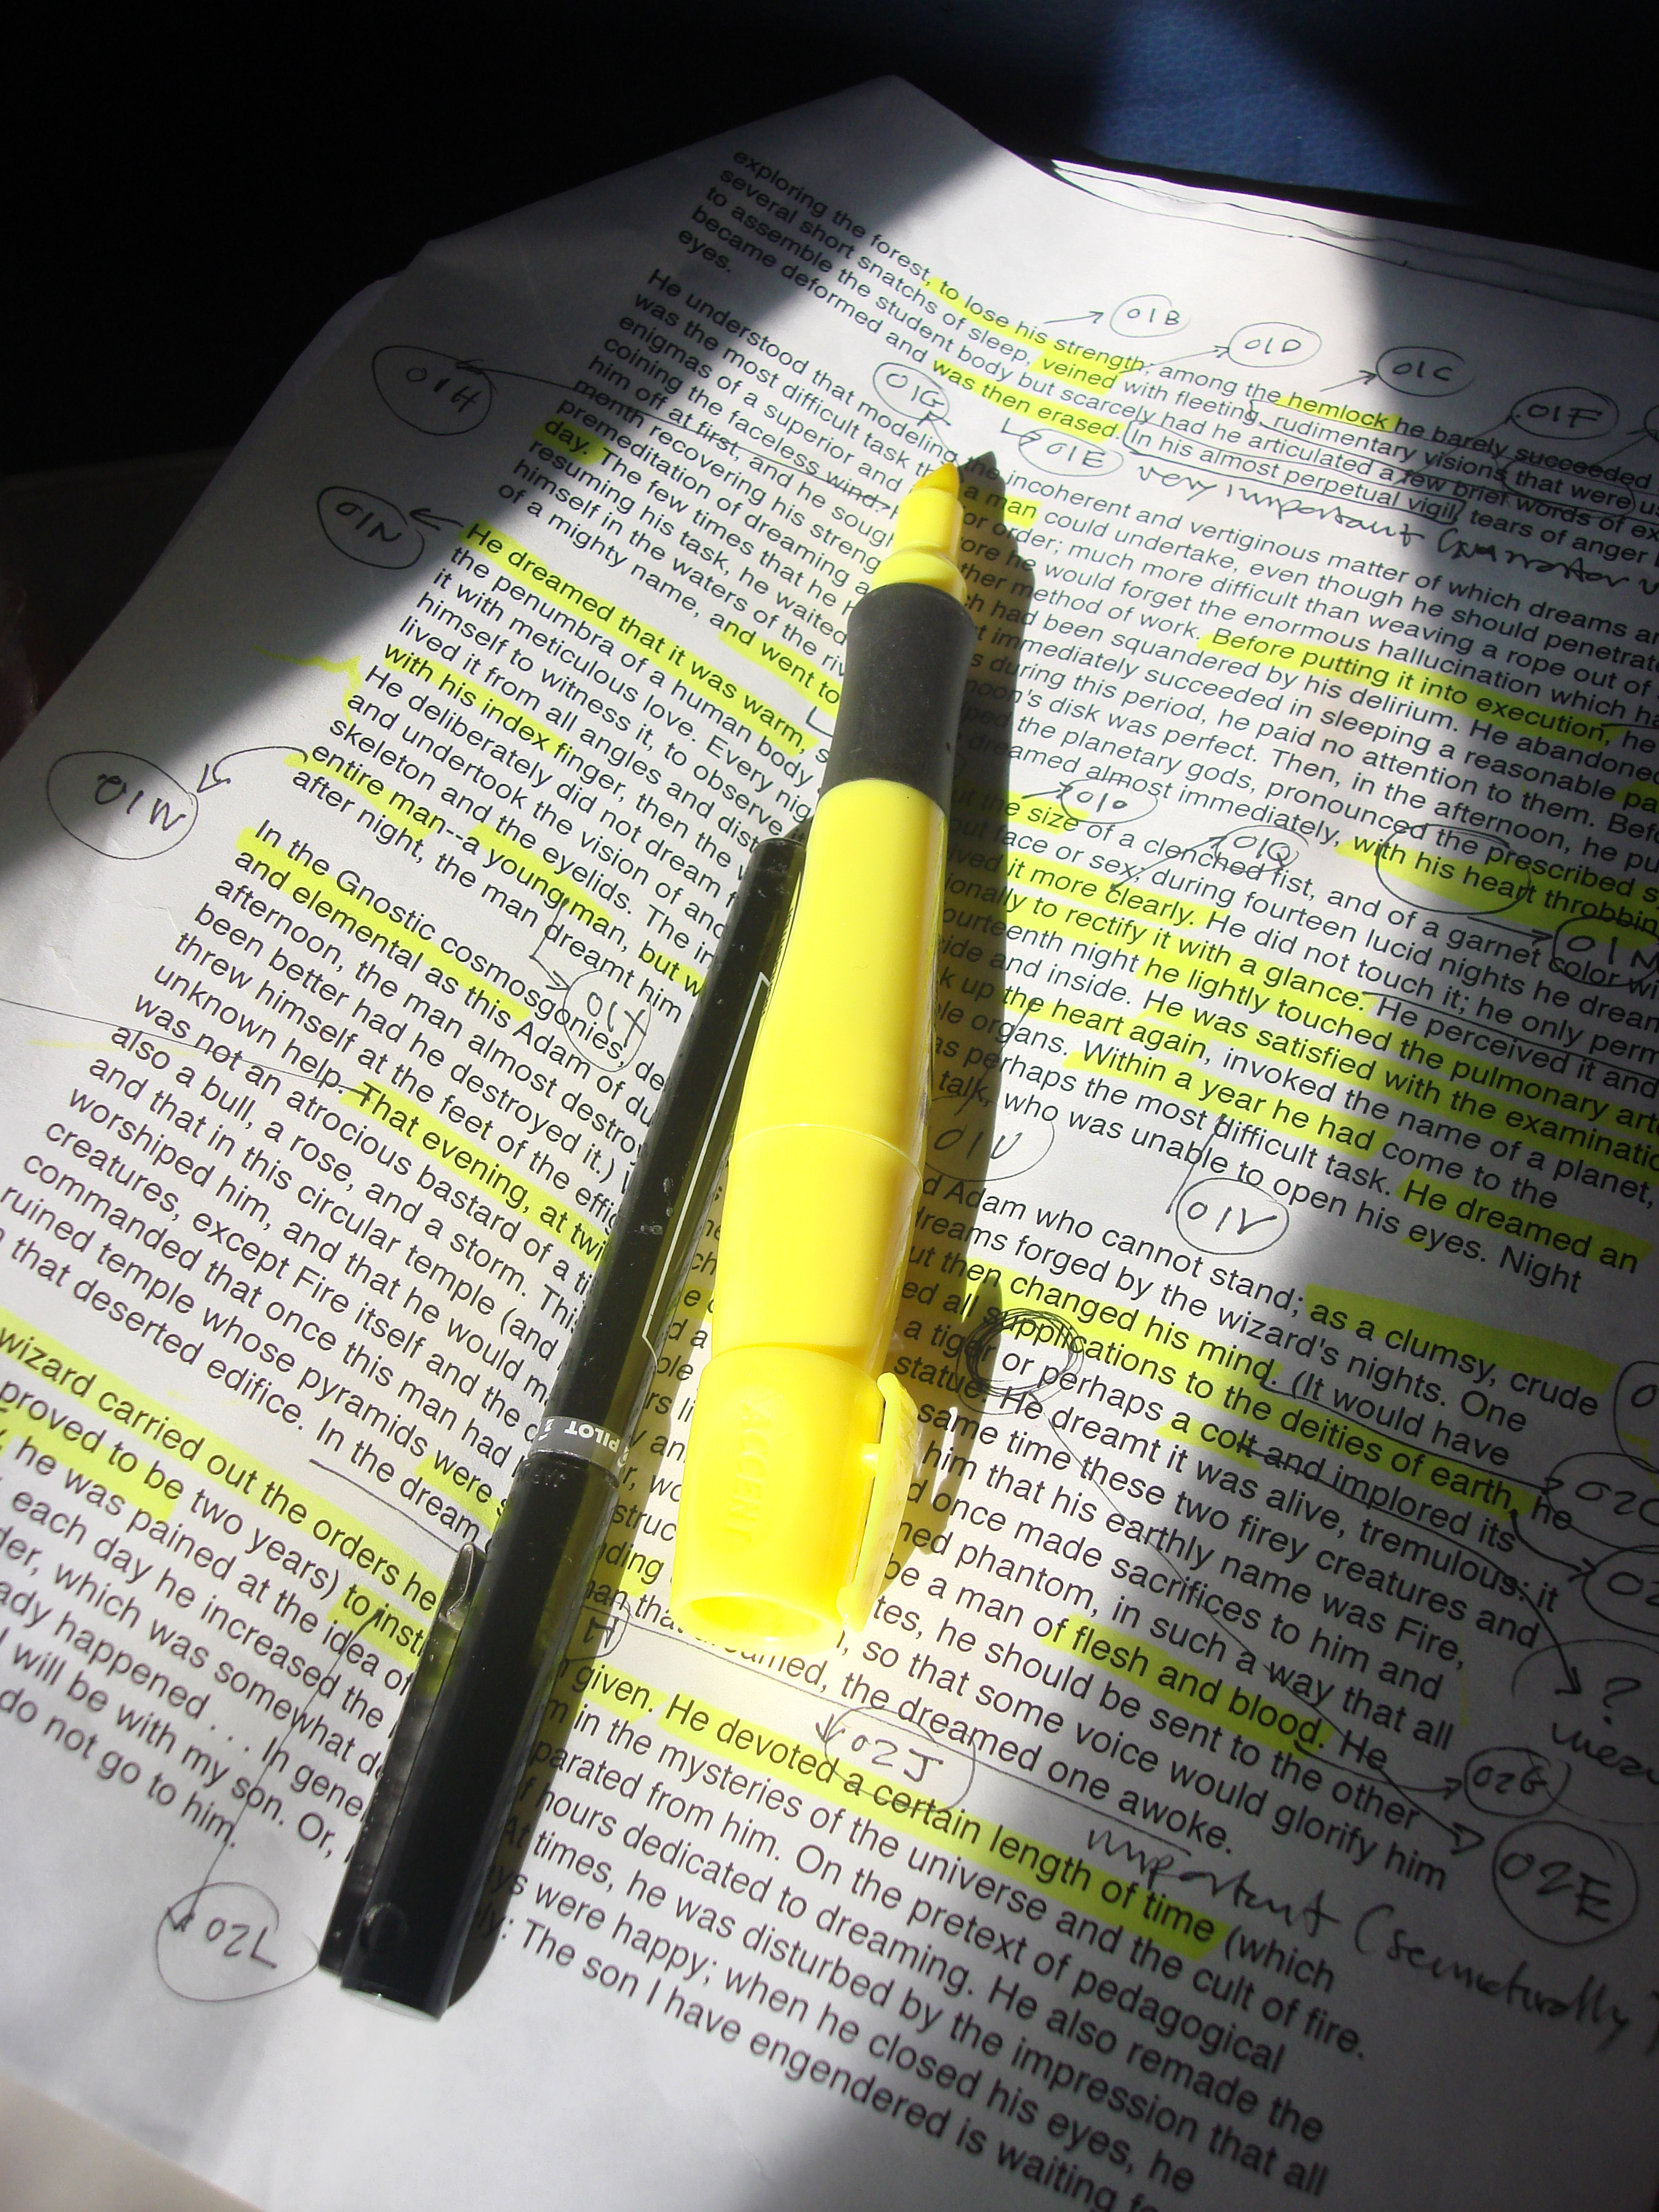
\includegraphics[width=\textwidth]{../img/textmarker}
  \end{columns}

  \vfill

  \hrulefill\\
  \hfill {\tiny Image by Guido ``random'' Alvarez, released as CC-BY-2.0}

\end{frame}

\subsection{Task 2: Understanding the Input/Output}

\begin{frame}
  \frametitle{Task 2: Reading the Input/Output}

  The Input Description is \alert{very important} (as we saw in 3n+1)

  \bigskip

  {\small
  \begin{itemize}
  \item What is the size of the data?
  \item What are the limits of the data?
  \item What is the format of the data?
  \item What is the stop condition?
  \end{itemize}
  }
\end{frame}

\begin{frame}
  \frametitle{Task 2: Input Size}

  The input size shows how big the problem gets.

  \begin{itemize}
  \item Small Problem: Full Search; Simulation;
  \item Big Problem: Complex Algorithms; Pruning;
  \end{itemize}

  \begin{block}{Keep in Mind!}
    \begin{itemize}
    \item The average time limit in UVA is 1-3 seconds.
    \item Expect maybe 10.000.000 operations per second.
    \end{itemize}
  \end{block}
\end{frame}

\begin{frame}
  \frametitle{Task 2: Input Size -- Examples}

  \begin{block}{n $<$ 24}
    Exponential algorithms will work (O($2^n$)).\\
    Or sometimes you can just calculate all solutions.
  \end{block}

  \begin{block}{n = 500}
    Cubic algorithms don't work anymore (O($n^3$) = 125.000.000)\\
    Maybe O($n^2\text{log}n$) will still work.
  \end{block}

  \begin{block}{n = 10.000}
    A square algorithm (O($n^2$)) might still work.\\
    But beware any big constants!
  \end{block}

  \begin{block}{n = 1.000.000}
    O($n$log$n$) = 13.000.000\\
    We might need a linear algorithm!
  \end{block}
\end{frame}

\begin{frame}
  \frametitle{Task 2: Input Format}

  Three common patterns for input format:
  \vfill

  \begin{itemize}
  \item Read $N$, then read $N$ queries;
  \bigskip

  \item Read until a special condition;
  \bigskip

  \item Read until EOF;
  \end{itemize}
\end{frame}

\begin{frame}[fragile]
  \frametitle{Task 2: Input Format}
  \begin{block}{}
    Read $N$, and then read $N$ queries;
    \bigskip

    Remember $N$ when calculating the size of the problem!
  \end{block}
  Example: \structure{Cost Cutting}

{\smaller
\begin{verbatim}
#include <iostream>
using namespace std;

int main()
{
    int n;
    cin >> n;

    for (; n > 0; n--)
    {
       // Do something
    }
}
\end{verbatim}}

\end{frame}

\begin{frame}[fragile]
  \frametitle{Task 2: Input Format}
  \begin{block}{}
    Read Until a Special Condition.

    Be careful: You can have \alert{many} queries before the condition!
  \end{block}

  Example: \structure{Request for Proposal:}\\
  The input ends with a line containing two zeroes.

{\smaller
\begin{verbatim}
int main()
{
   cin >> n >> p;
   while (n!=0 || p!=0)
   {
       // do something!
       cin >> n >> p;
   }
}
\end{verbatim}}
\end{frame}

\begin{frame}[fragile]
  \frametitle{Task 2: Input Format}
  \begin{block}{}
    Read until EOF.
    \bigskip

    Functions in C and Java return FALSE when they read EOF. Python requires
    an exception. Very common in UVA.
  \end{block}
  Example: \structure{3N+1 Problem, Jolly Jumpers}

{\smaller
\begin{verbatim}
int main()
{
    int a, b;
    while (cin >> a >> b;)
    {
        // Do something!
    }
}
\end{verbatim}
}
\end{frame}

\begin{frame}
  \frametitle{Task 2: Output Format}

  The UVA judge decides the result based on a simple \alert{diff}.
  \bigskip

  Be \alert{very careful} that the output is exactly right!

  \vspace{3cm}

  \begin{columns}
    \column{0.2\textwidth}
    
\includegraphics[width=1\textwidth]{../img/angryclient}
    \column{0.7\textwidth} \emph{The Judge is like an angry client. It
      wants the output EXACTLY how it stated.}
  \end{columns}
\end{frame}

\begin{frame}
  \frametitle{Task 2: Output Format -- Checklist}

  
\includegraphics[width=0.15\textwidth]{../img/angryclient}
  \begin{enumerate}
    \item DID YOU REMOVE DEBUG OUTPUT?
    \item DID YOU REMOVE DEBUG OUTPUT?
    \smallskip

    \item Easy mistakes: UPPERCASE x lowercase, spleling mitsakes;
    \item Boring mistakes: plural: 1 hour \structure{or} 2 hours;
    \item What is the precision of \structure{float}? (3.051 \structure{or} 3.05)
    \item Round up or Round down? (3.62 $\rightarrow$ 3 \structure{or} 4)
    \item Multiple solutions: Which one do you output\\ (usually ortographical sort)
  \end{enumerate}
\end{frame}


\begin{frame}
  \frametitle{Task 2: Input/Output -- Traps!}

  \begin{block}{Example: 3n+1 Problem}
    \begin{itemize}
    \item $i$ and $j$ can come in any order.
    \end{itemize}
  \end{block}

  \begin{block}{Common Traps}
    \begin{itemize}
    \item Negative numbers, zeros;
    \item Duplicated input, empty input;
    \item No solutions, multiple solutions;
    \item Other special cases;
    \end{itemize}
  \end{block}
  \vfill

  \hfill 
\includegraphics[width=0.25\textwidth]{../img/trap}
\end{frame}

\subsection{Task 3: Choosing the algorithm}


\begin{frame}
  \frametitle{Task 3: Choosing the algorithm}
  The important part of choosing the algorithm is \alert{counting the time}
  \bigskip

  \begin{itemize}
    \item An algorithm with $k$-nested loops of and $n$ commands
      has $O(nk)$ complexity;
    \item A recursive algorithm with $b$ recursive calls per level, and $L$
      levels, it should have $O(bL)$ complexity;
    \item An algorithm with $p$ nested loops of size $n$ is $O(n^p)$
    \item An algorithm processing a $n*n$ matrix in O(k) per cell runs
      in $O(kn^2)$ time.
  \end{itemize}

  \bigskip

  Use \alert{pruning} to reduce the complexity of your algorithm!\\
  Also don't forget the number of queries!
\end{frame}

\begin{frame}[fragile]
  \frametitle{Task 3: Example of Pruning -- 8 queen problem}

  \hfill 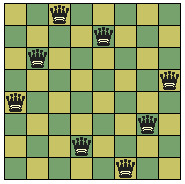
\includegraphics[width=0.2\textwidth]{../img/8queen}

  You want to find a position for 8 queens where no queen attack another queen.

  \bigskip

\begin{verbatim}
Solution 1: All options:
Queen1: a1 or a2 or a3 or a4 ... or h5 or h6 or h7 or h8
Queen2: Same as Queen 1
Queen3: Same as Queen 2
...
Queen8: Same as Queen 7

Total Solutions: 64 x 64 x 64 x 64 = 64^8 ~ 10^14
\end{verbatim}
\end{frame}

\begin{frame}[fragile]
  \frametitle{Task 3: Example of Pruning -- 8 queen problem}

  \hfill 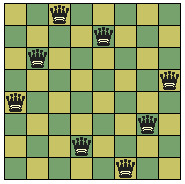
\includegraphics[width=0.2\textwidth]{../img/8queen}

  You want to find a position for 8 queens where no queen attack another queen.

  \bigskip

\begin{verbatim}
Solution 2: One queen / column
Queen1: a1 or a2 or a3 ...
Queen2: b1 or b2 or b3 ...
Queen3: c1 or c2 or c3 ...
...
Queen8: h1 or h2 or h3 ...

Total Solutions: 8 x 8 x 8 ... = 8^8 ~ 10^7
\end{verbatim}
\end{frame}

\begin{frame}[fragile]
  \frametitle{Task 3: Example of Pruning -- 8 queen problem}

  \hfill 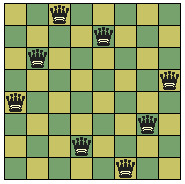
\includegraphics[width=0.2\textwidth]{../img/8queen}

  You want to find a position for 8 queens where no queen attack another queen.

  \bigskip

\begin{verbatim}
Solution 3: One queen / row x column
If Q1 is a1, Q2 in b2, Q3 must be c3-7...

A solution is the order of rows: Ex: 1-3-5-2-7-4-8-6

Total Solutions: 8 x 7 x 6 x 5 ... = 40320
\end{verbatim}
\end{frame}

\subsection{Task 4: Coding}

\begin{frame}
  \frametitle{Task 4: Coding}

  Do you understand \structure{The Problem} and \structure{The Algorithm}?

  \bigskip

  {\bf NOW} you can start writing your program.

  \vfill

  \begin{block}{}
    If you start your program before you understand the solution, you
    will create many more bugs.
  \end{block}
\end{frame}

\begin{frame}
  \frametitle{Task 4: Coding}
  \begin{exampleblock}{Hint 1: ``The Library''}
    Create a file with code examples that you often use.
    \begin{itemize}
    \item Input/output functions;
    \item Common data structures;
    \item Difficult algorithms;
    \end{itemize}
   \end{exampleblock}

   \begin{block}{Hint 2: Use paper}
    \begin{itemize}
    \item Writing your idea on paper help you visualize;
    \item Sometimes you can find bugs this way;
    \end{itemize}
  \end{block}
\end{frame}

\begin{frame}
  \frametitle{Task 4: Coding}

  \begin{block}{Hint 3: Programmer Efficiency}
    Everyone knows about \structure{CPU efficiency} or
    \structure{Memory efficiency}.

    \bigskip

    But \structure{Programmer Efficiency} is very important too: Don't
    get \structure{tired/confused!}
  \end{block}

  \vfill

  \begin{itemize}
  \item Use standard library and macros;
  \item Your program just need to solve THIS problem;
  \item Use simple structures and algorithms;
  \item TDD mindset;
  \end{itemize}
\end{frame}


\subsection{Testing}
\begin{frame}
  \frametitle{Task 5,6: Test and Hidden Data}

  The example data {\bf is not} all the data!

  \bigskip

  \begin{columns}
    \column{0.45\textwidth}
    \begin{exampleblock}{Example Data}
      \begin{itemize}
      \item Useful to test input/output;
      \item Read the example data to understand the problem;
      \end{itemize}
    \end{exampleblock}
    \column{0.45\textwidth}
    \begin{alertblock}{Hidden Data}
      \begin{itemize}
      \item Used by the UVA judge;
      \item Contain bigger data sets;
      \item Includes special cases;
      \end{itemize}
    \end{alertblock}
  \end{columns}

  \medskip

  Generate your own set of hidden data before submitting!
\end{frame}

\begin{frame}
  \frametitle{What data to generate?}

  \begin{itemize}
  \item Datas with multiple entries (to check for initialization);
  \item Datas with maximum size (can be trivial cases);
  \item Random data;
  \item Border cases (maximum and minimum values in input range);
  \item Worst cases (depends on the problem);
  \end{itemize}
\end{frame}

\begin{frame}
  \frametitle{The uDebug Website}

  \begin{center}
    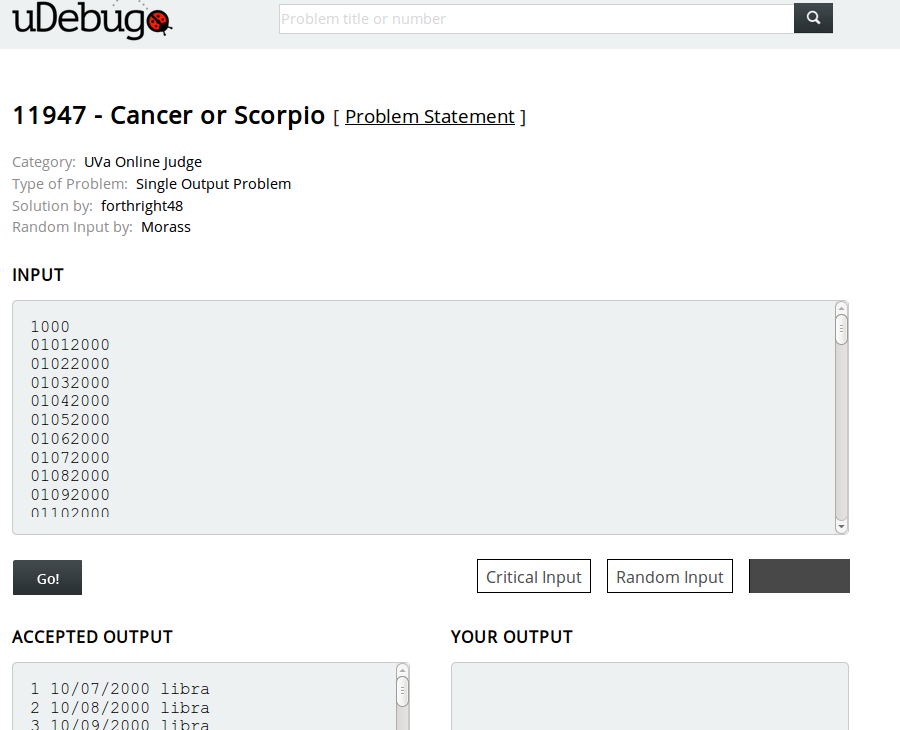
\includegraphics[width=0.8\textwidth]{../img/udebug_big}
  \end{center}
\end{frame}

\section{Conclusion}
\subsection{The End}
\begin{frame}
  \frametitle{To Summarize}
  Mental framework to solve problems:
  \begin{enumerate}
  \item Read the problem carefully to avoid traps;
  \item Think of the algorithm and data structure;
  \item Keep the size of the problem in mind;
  \item Keep your code simple;
  \item Create special test cases;
  \end{enumerate}

  \vfill

  \begin{block}{}
    Now go solve the other problems!
  \end{block}
\end{frame}

\begin{frame}
  \frametitle{Thanks for Listening!}
  \begin{center}
    Any questions?
  \end{center}
\end{frame}

\begin{frame}
  \frametitle{BONUS -- Calculating Complexity in Research Experiments}
\end{frame}

\begin{frame}
  \frametitle{BONUS -- A very simple program}

  \begin{block}{Ackermann's Function}
    \begin{eqnarray*}
      A(m,n) = & n+1 & \text{if } m = 0\\
      & A(m-1,1) & \text{if } m > 0, n = 0\\
      & A(m-1,A(m,n-1)) & \text{if } m > 0, n > 0\\
    \end{eqnarray*}
  \end{block}

  \begin{itemize}
    \item $A(0,n) = 1$ step
    \item $A(1,n) = 2n+2$ steps
    \item $A(2,n) = n^2$ steps
    \item $A(3,n) = 2^{n+3}-3$ \alert{!}
    \item $A(4,n) = 2^{2^{...^2}}-3$ \alert{!!!} (exponential tower of n+3)
    \item $A(5,n) = $ \alert{!!!!!!!!!!!!}
  \end{itemize}
\end{frame}


\end{document}
